\documentclass[a4paper]{iacas}

\usepackage{cite}
\usepackage{hyperref}% embedding hyperlinks [must be loaded after dropping]
\usepackage{amsmath,amsthm,amssymb,amsfonts,latexsym,mathrsfs,wasysym}
\usepackage{marvosym}
\usepackage{subcaption}
\usepackage{soul,color}
\usepackage{threeparttable}% tables with footnotes
\usepackage{dcolumn}% decimal-aligned tabular math columns
\usepackage{float}
\usepackage{graphicx}
\usepackage{accents}
\usepackage{tikz}
\usepackage{lastpage}
\usepackage{fancyhdr}
\usepackage{color}
\usepackage{cancel}
\usepackage{setspace}
\usepackage{multirow}
%\doublespacing
% or:
\onehalfspacing
%\usepackage[T1]{fontenc}
%\usepackage{bigfoot} % to allow verbatim in footnote
\usepackage[framed,numbered]{matlab-prettifier}
\pagestyle{plain}
%\usepackage[hebrew,english]{babel}
\usetikzlibrary{shapes.geometric, arrows, calc}

\newcolumntype{d}{D{.}{.}{-1}}
\graphicspath{{figures/}}

% define some commands to maintain consistency
\newcommand{\pkg}[1]{\texttt{#1}}
\newcommand{\cls}[1]{\textsf{#1}}
\newcommand{\file}[1]{\texttt{#1}}
\newcommand{\sgn}[1]{\operatorname{sgn}\left(#1\right)}
\newcommand{\sat}[1]{\operatorname{sat}\left(#1\right)}
\newcommand{\rrule}[1]{\rule[#1]{0pt}{0pt}}
\newcommand{\fracds}[2]{\frac{\displaystyle #1\rrule{-0.2em}}{\displaystyle #2\rrule{1em}}}
\newcommand{\figref}[1]{Fig.~\ref{#1}}
\newcommand{\ubar}[1]{\underaccent{\bar}{#1}}
\newcommand{\norm}[1]{\lvert \lvert \vec #1 \rvert \rvert}

%diffeomorphism

\begin{document}


\begin{center}
	\large Algorithms and Application in Computer Vision - 046746
\end{center}
\begin{center}
	\large\textbf{Homework \#3}
\end{center}


\begin{tabular}{l}
	\\
	{\bf\textit{Alexander Shender 328626114}} \\
	{\bf\textit{Vladimir Tchuiev 309206795}} \\
	Technion - Israel Institute of Technology
\end{tabular}


%\newpage
\vspace{2em}

\section{Eigen-Faces and PCA for face recognition}


\subsection{Section 1}

We computed the average image from the grayscale training set of face images. The result is presented in Fig.~\ref{fig:100}. The resulting average image is a vague male face; notice the black lines on the top and bottom of the average image, they are presented in all training set images.

\begin{figure}[!htbp]
	\centering
	\begin{subfigure}[b]{0.6\textwidth}
		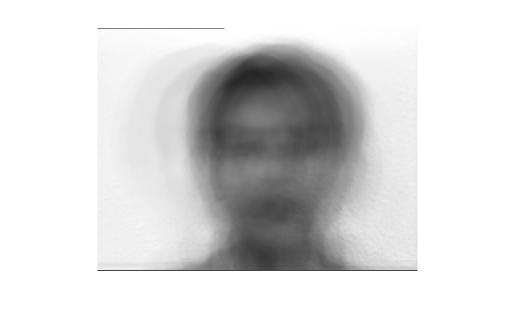
\includegraphics[width=\textwidth]{101.jpg}
		\label{fig:101}
	\end{subfigure}
	
	\caption{Average image from training set.}
	\label{fig:100}
\end{figure}

\subsection{Section 2}

From all the training set images, we computed the 25 eigenfaces with the largest eigenvalues. We flattened each $243 \times 320$ pixel image into a vector with $77760$ elements. We concatenated all these vectors into a single $A \in \mathbb{R}^{77760 \times 150}$ matrix. In order to compute the eigenfaces, we will have to create the matrix $AA^T \in \mathbb{R}^{77760 \times 77760}$, the covariance matrix that corresponds to each pixel, and compute its eigenvalues and eigenvectors. This matrix is extremely large and computing its eigenvectors is costly, thus we will compute the eigenvalues and vectors of $A^TA$ and use it to compute the eigenvectors of $AA^T$ instead:
%
\begin{equation}
A^TAx = x\lambda
\end{equation}
%
where $\lambda$ is the eigenvalue of $A^TA$ and $x$ is the corresponding eigenvector. Then:
%
\begin{equation}
(AA^T)(Ax) = (Ax)\lambda
\end{equation}
%
thus $\lambda$ is a (non-zero) eigenvalue of $AA^T$ as well, and its corresponding eigenvector is $Ax$. Therefore we only need to compute the eigenvectors of $A^TA \in \mathbb{R}^{150 \times 150}$, which is a significantly more manageable task.

In Fig.~\ref{fig:200} we present the 5 eigenfaces with the largest eigenvalues. The images are normalized such that the 0 value is 50 percent gray.

\begin{figure}[!htbp]
	\centering
	\begin{subfigure}[b]{0.18\textwidth}
		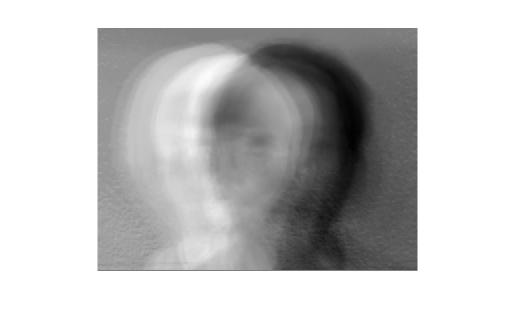
\includegraphics[width=\textwidth]{201.jpg}
		\caption{}
		\label{fig:201}
	\end{subfigure}
	%
	\begin{subfigure}[b]{0.18\textwidth}
		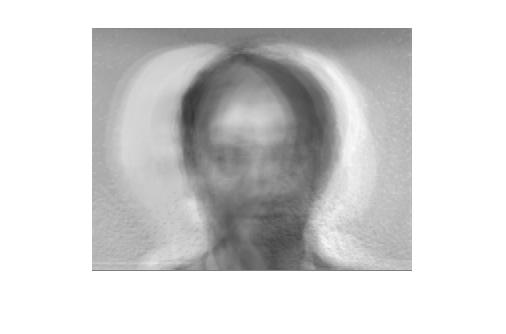
\includegraphics[width=\textwidth]{202.jpg}
		\caption{}
		\label{fig:202}
	\end{subfigure}
	%
	\begin{subfigure}[b]{0.18\textwidth}
		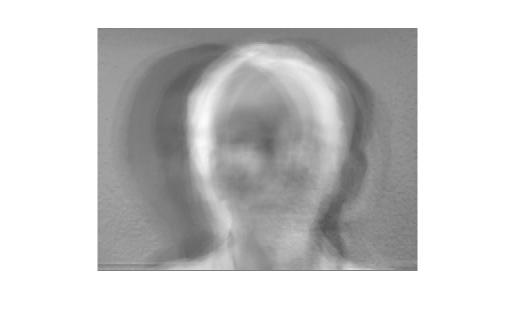
\includegraphics[width=\textwidth]{203.jpg}
		\caption{}
		\label{fig:203}
	\end{subfigure}
	%
	\begin{subfigure}[b]{0.18\textwidth}
		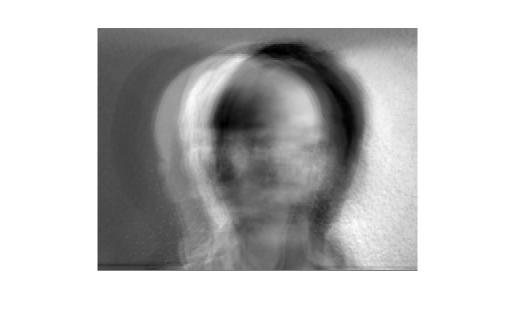
\includegraphics[width=\textwidth]{204.jpg}
		\caption{}
		\label{fig:204}
	\end{subfigure}
	%
	\begin{subfigure}[b]{0.18\textwidth}
		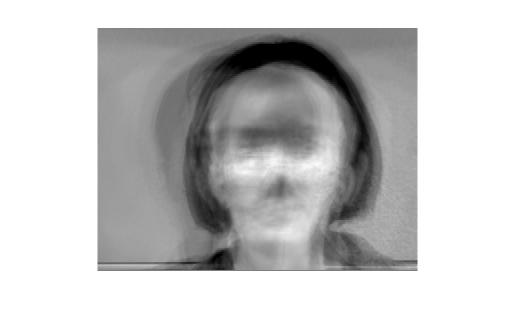
\includegraphics[width=\textwidth]{205.jpg}
		\caption{}
		\label{fig:205}
	\end{subfigure}
	
	\caption{From left to right: eigenfaces with largest eigenvalues in descending order.}
	\label{fig:200}
\end{figure}

\subsection{Section 3}

In this section we reconstruct the training set images using the reduced representation, and reconstruction errors. Note that for the reconstruction we normalized the $W$ matrix of eigenfaces such that $W^TW = I$.

In Fig.~\ref{fig:3000} we present training set images on the left column, compared to a reconstruction using 25 highest eigenvalue eigenfaces. We can see that the reconstruction is lacking detail, but overall pretty close to the training set. If we were to take all 150 eigenvalues, we would have a perfect reconstruction.

\begin{figure}[!htbp]
	\centering
	\begin{subfigure}[b]{0.4\textwidth}
		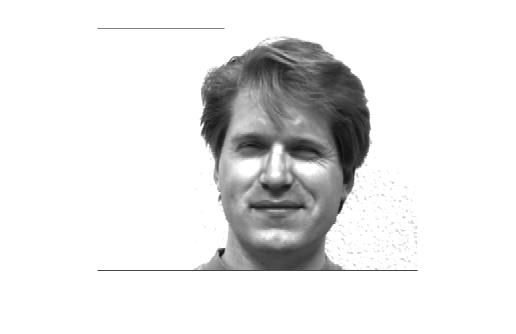
\includegraphics[width=\textwidth]{3102.jpg}
		\caption{}
		\label{fig:3102}
	\end{subfigure}
	%
	\begin{subfigure}[b]{0.4\textwidth}
		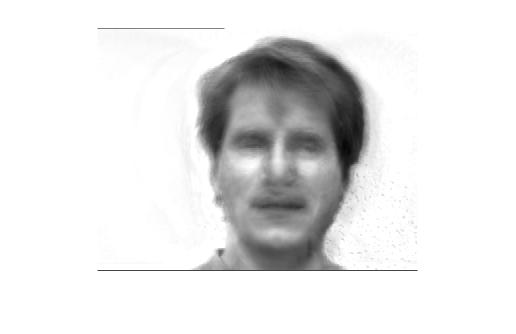
\includegraphics[width=\textwidth]{3101.jpg}
		\caption{}
		\label{fig:3101}
	\end{subfigure}
	
	\begin{subfigure}[b]{0.4\textwidth}
		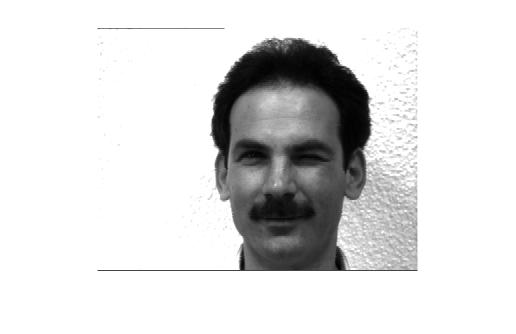
\includegraphics[width=\textwidth]{3202.jpg}
		\caption{}
		\label{fig:3202}
	\end{subfigure}
	%
	\begin{subfigure}[b]{0.4\textwidth}
		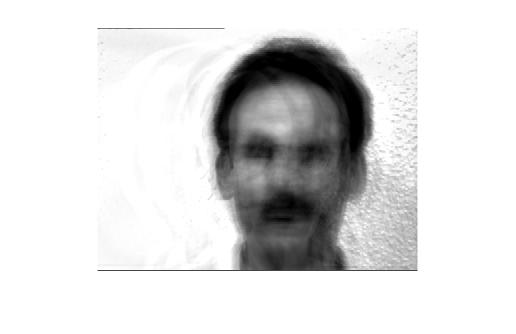
\includegraphics[width=\textwidth]{3201.jpg}
		\caption{}
		\label{fig:3201}
	\end{subfigure}
	
	\begin{subfigure}[b]{0.4\textwidth}
		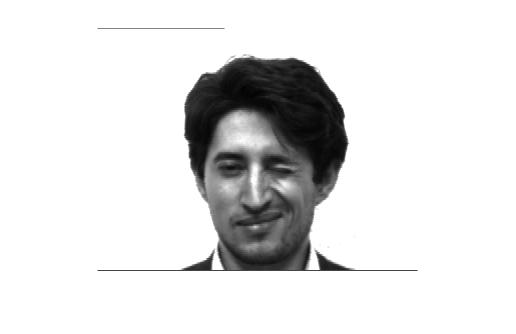
\includegraphics[width=\textwidth]{3302.jpg}
		\caption{}
		\label{fig:3302}
	\end{subfigure}
	%
	\begin{subfigure}[b]{0.4\textwidth}
		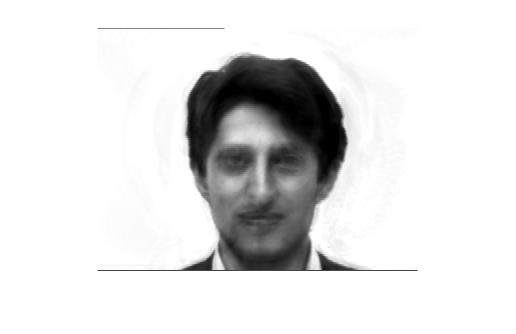
\includegraphics[width=\textwidth]{3301.jpg}
		\caption{}
		\label{fig:3301}
	\end{subfigure}
	
	\caption{Training set; Left column: original images from training set. Right column: image reconstruction based on 25 largest eigenvalue eigenfaces.}
	\label{fig:3000}
\end{figure}

In Fig.~\ref{fig:300} we present a graph of errors relative to the serial number of the image. We can see that dynamic range RMSE error has a significantly smaller value than RMSE error, as it tends to normalize large value swings. The average RMSE error is $79.54 \cdot 10^{-3}$, while the average Dynamic Range RMSE error is $3.337 \cdot 10^{-3}$.

\begin{figure}[!htbp]
	\centering
	\begin{subfigure}[b]{0.5\textwidth}
		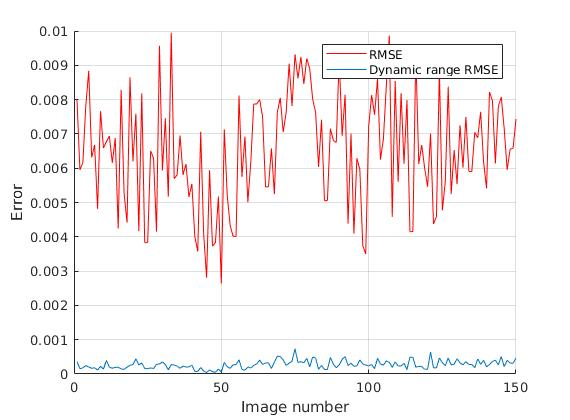
\includegraphics[width=\textwidth]{310.jpg}
		\label{fig:310}
	\end{subfigure}
	
	\caption{Training set; RMSE and Dynamic Range RMSE errors vs. image serial number.}
	\label{fig:300}
\end{figure}

\subsection{Section 4}

In this section we reconstruct the test set images using the reduced representation, and reconstruction errors.

In Fig.~\ref{fig:4000} we present test set images on the left column, compared to a reconstruction using 25 highest eigenvalue eigenfaces trained on the original 150 images. We can see that the reconstruction captures faces' general form well but fails to reconstruct objects that are not faces, such as the Google Chrome symbol. This reconstruction is enough for classifying faces relatively well, as the classification accuracy we reached for the eigenfaces algorithm is \textbf{81.82 percent}. We performed the classification over all face images, and ignored the non-face images as the inferred class has no meaning for these cases.

\begin{figure}[!htbp]
	\centering
	
	\begin{subfigure}[b]{0.4\textwidth}
		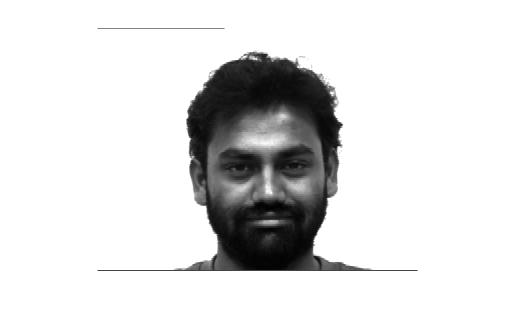
\includegraphics[width=\textwidth]{4102.jpg}
		\caption{}
		\label{fig:4102}
	\end{subfigure}
	%
	\begin{subfigure}[b]{0.4\textwidth}
		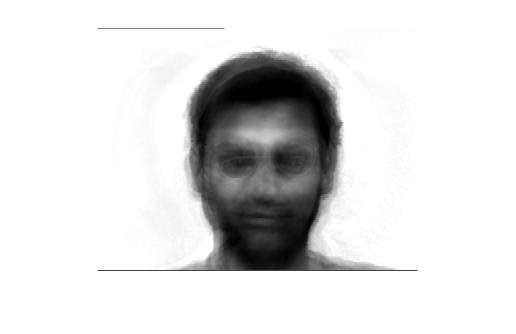
\includegraphics[width=\textwidth]{4101.jpg}
		\caption{}
		\label{fig:4101}
	\end{subfigure}
	
	\begin{subfigure}[b]{0.4\textwidth}
		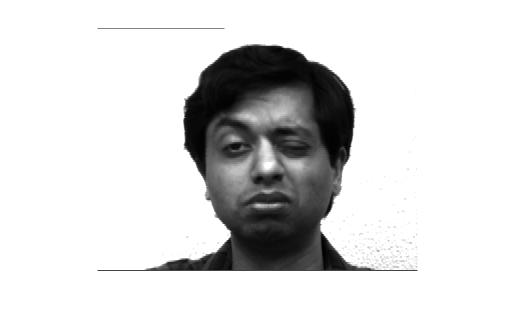
\includegraphics[width=\textwidth]{4152.jpg}
		\caption{}
		\label{fig:4152}
	\end{subfigure}
	%
	\begin{subfigure}[b]{0.4\textwidth}
		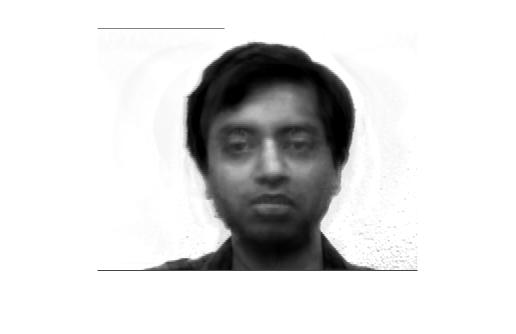
\includegraphics[width=\textwidth]{4151.jpg}
		\caption{}
		\label{fig:4151}
	\end{subfigure}
	
	\begin{subfigure}[b]{0.4\textwidth}
		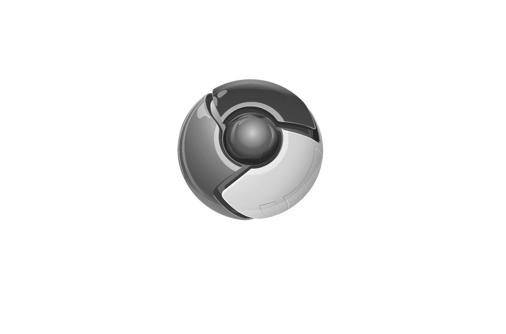
\includegraphics[width=\textwidth]{4012.jpg}
		\caption{}
		\label{fig:4012}
	\end{subfigure}
	%
	\begin{subfigure}[b]{0.4\textwidth}
		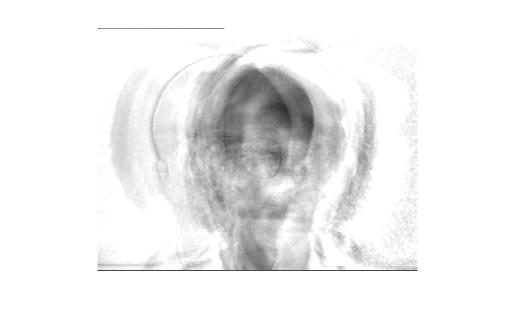
\includegraphics[width=\textwidth]{4011.jpg}
		\caption{}
		\label{fig:4011}
	\end{subfigure}
	
	\caption{Test set; Left column: original images from training set. Right column: image reconstruction based on 25 largest eigenvalue eigenfaces.}
	\label{fig:4000}
\end{figure}

In Fig.~\ref{fig:400} we present a graph of errors relative to the serial number of the image. The average RMSE error is $143.8 \cdot 10^{-3}$, while the average Dynamic Range RMSE error is $6.890 \cdot 10^{-3}$. As expected, the reconstruction error for the test set is significantly larger than the training set, also due to the fact that the test set contains images that are very far from the training set (high model uncertainty).

\begin{figure}[!htbp]
	\centering
	\begin{subfigure}[b]{0.5\textwidth}
		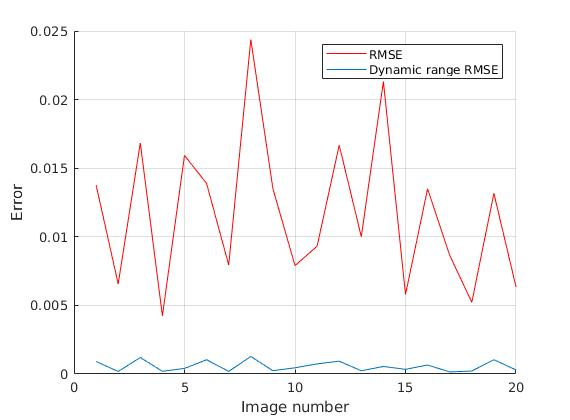
\includegraphics[width=\textwidth]{410.jpg}
		\label{fig:410}
	\end{subfigure}
	
	\caption{Test set; RMSE and Dynamic Range RMSE errors vs. image serial number.}
	\label{fig:400}
\end{figure}
















\newpage
\section{Fisher Linear Discriminant for face recognition}


\subsection{}
The stub code 'fishertrain.m' was completed as described in the presented steps. The matrix $W_{fld}$ was calculated using the generalized eigenvalues decomposition (GED), containing $c-1$ largest eigenvectors. The resulting Fisher basis is indeed: $$W=W_{pca}W_{fld}$$. Explanation: for the Fisher basis, we did not use the original image vectors (which are of the size of $234*320=77760$), in order to avoid huge matrixes $S_{B}$ and $S_{W}$. We have used instead their representation using the PCA basis, which was already calculated. By setting the size of the basis for PCA to be $r = N-C$, the scatter matrixes   $S_{B}$ and $S_{W}$  have resulted in being the size of [r x r] (scatter matrixes are square matrixes, [r x r], where r - number of dimensions in data). Thus, the $W_{fld}$ matrix, after taking $c-1$ eigenvectors with largest eigenvalues, is of the size [r (c-1)]. The $W_{pca}$, on the other hand, projects the image vector to a vector of size r. Thus, its size is [77760 x r].  Eventually, we obtain matrix $W$, which projects the image vector first on the PCA basis, and then on the $c-1$ strongest eigenvectors of the GED. Thus, we obtain:
$$W = W_{pca}{[} 77760 \times r\ {]}W_{fld}{[} r \times c-1 {]} = W{[} 77760 \times c-1 {]}$$
And $W$ projects the image vector to a Fisher basis.

\subsection{}
By using the parameter $c=15$ we obtain the sizes for the matrixes (for sanity check)

\begin{align*}
R =& N - c = 135 \\
S_{B}, S_{W} \in& [135 \times 135] \\
W_{pca} \in&  [77760 \times 135] \\
W_{fld} \in&  [135 \times 14] \\
W \in& [77760 \times 14] 
\end{align*}
Thus, we project each image on a vector of size 14. 
Using the code from the section A, we calculate the representation errors for the training set and for the test set.
\newline

\vskip 0.1in
\begin{minipage}{\linewidth}
	\centering
	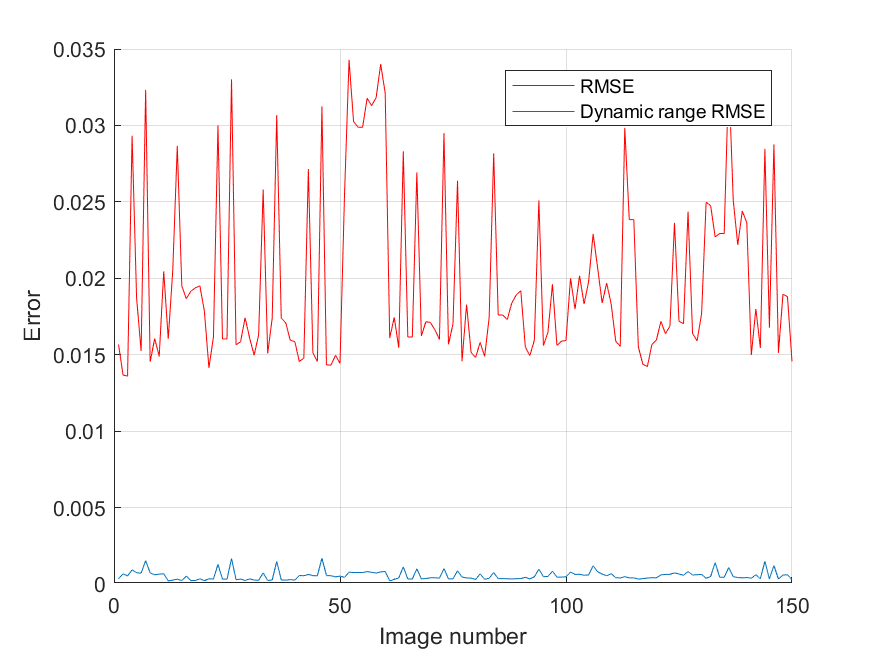
\includegraphics[scale=0.9]{imgs2/rmse_train.png}
	\captionof{figure}{Training set reconstruction errors}
	\label{fig_1}
\end{minipage}
\vskip 0.1in
\begin{minipage}{\linewidth}
	\centering
	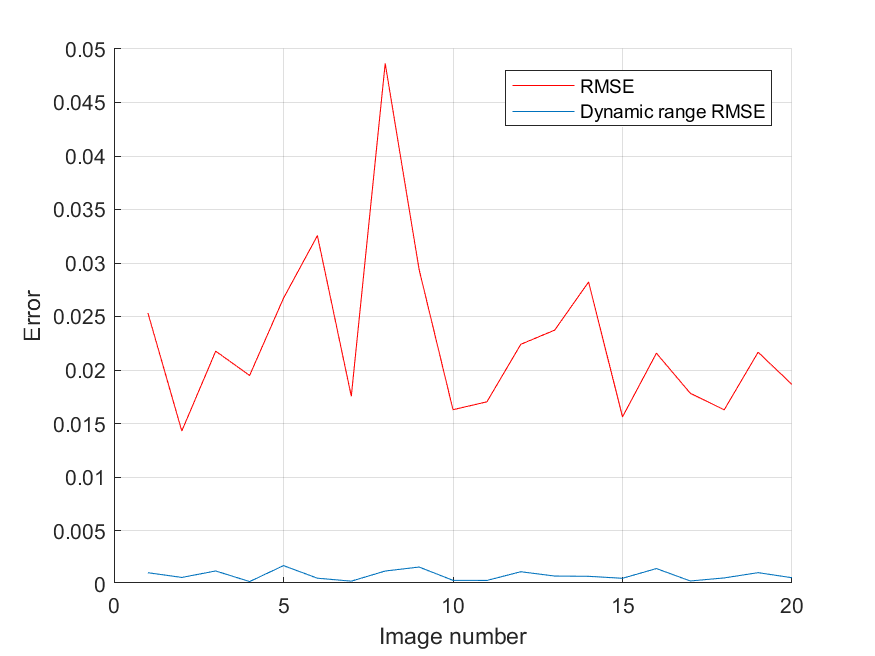
\includegraphics[scale=0.9]{imgs2/rmse_test.png}
	\captionof{figure}{Test set reconstruction errors}
	\label{fig_1}
\end{minipage}
\vskip 0.1in

We can see that the reconstuction errors are larger than the reconstruction from the PCA basis alone from the previous section. We can explain this by the fact the the representation vector from the Section A was of size 25, while in this section we use the representation of size 14.

 \subsection{}
Using the FLD, we achieve a fantastic classification rate of 100\%! This demonstrates that using the Fisher Basis, we achieve better classification of the dataset. The explanation can be found in numerous resources.
\newline
The PCA finds the most accurate representation of the data, in a lower dimensional space. It finds the directions of maximum variances, but those may be not so good for classification, since they may be similar for different classes. What Fisher Linear Discriminator does is finds a projection of the representation of the data, where the classes are separated in an optimal way - where the separation is good. This is done my maximizing the between-classes scatter matrix, and minimizing the within-classes scatter matrix.  Good separation means good classification - there is less overlapping of the classes representations on the projection subspace.


\end{document}




















